\documentclass[main.tex]{subfiles}
\begin{document}


% BTK: Waurm wurde so evaluiert ? Damit es wissenschaftlich ist.  
\chapter{Evaluation}

Ob ein Framework oder ein OSRE performant ist, kann kaum der Literatur entnommen werden. Auch Benchmarks stossen dabei an ihre Grenzen, wenn es darum geht, Vergleiche zwischen Frameworks zu machen, die je nach Einsatzgebiet verschiedene Stärken oder Schwächen aufweisen können. Dadurch kann eine objektive Aussage zwar wahr sein, sie ist womöglich aber für das eigene Projekt nicht aussreichend oder sogar falsch. Es wurde entschieden, einen eigenen Prototypen zu erstellen, den es in dieser Arbeit zu evaluieren gilt. 

Für die Evaluation wurde bestimmt, die Prototypen abwechslungsweise auf die PaaS einzusetzen, um diese separat voneinander analysieren zu können. Gegen die eingesetzten Prototypen wurden automatische Lasttest durchgeführt. Da die Performance-Messungen mehrmals zu erheben waren, wurde vorgängig ein Testplan erstellt. Damit konnten die Tests vorgängig konfiguriert und automatisiert durchgeführt werden. Die wichtigsten Performance-Messungen wurden einerseits mit dem Testtool JMeter generiert und andererseits mithilfe der Logs auf der PaaS erhoben. Dank der Konsolidierung dieser Dateien konnten Rückschlüsse auf die Performance gezogen werden.

Die Evaluation gliedert sich in drei Teile (siehe Abbildung \ref{figure:evaluationsAblauf}). Diese Teile werden in den folgenden Kapiteln näher erläutert.

\begin{figure}[h]
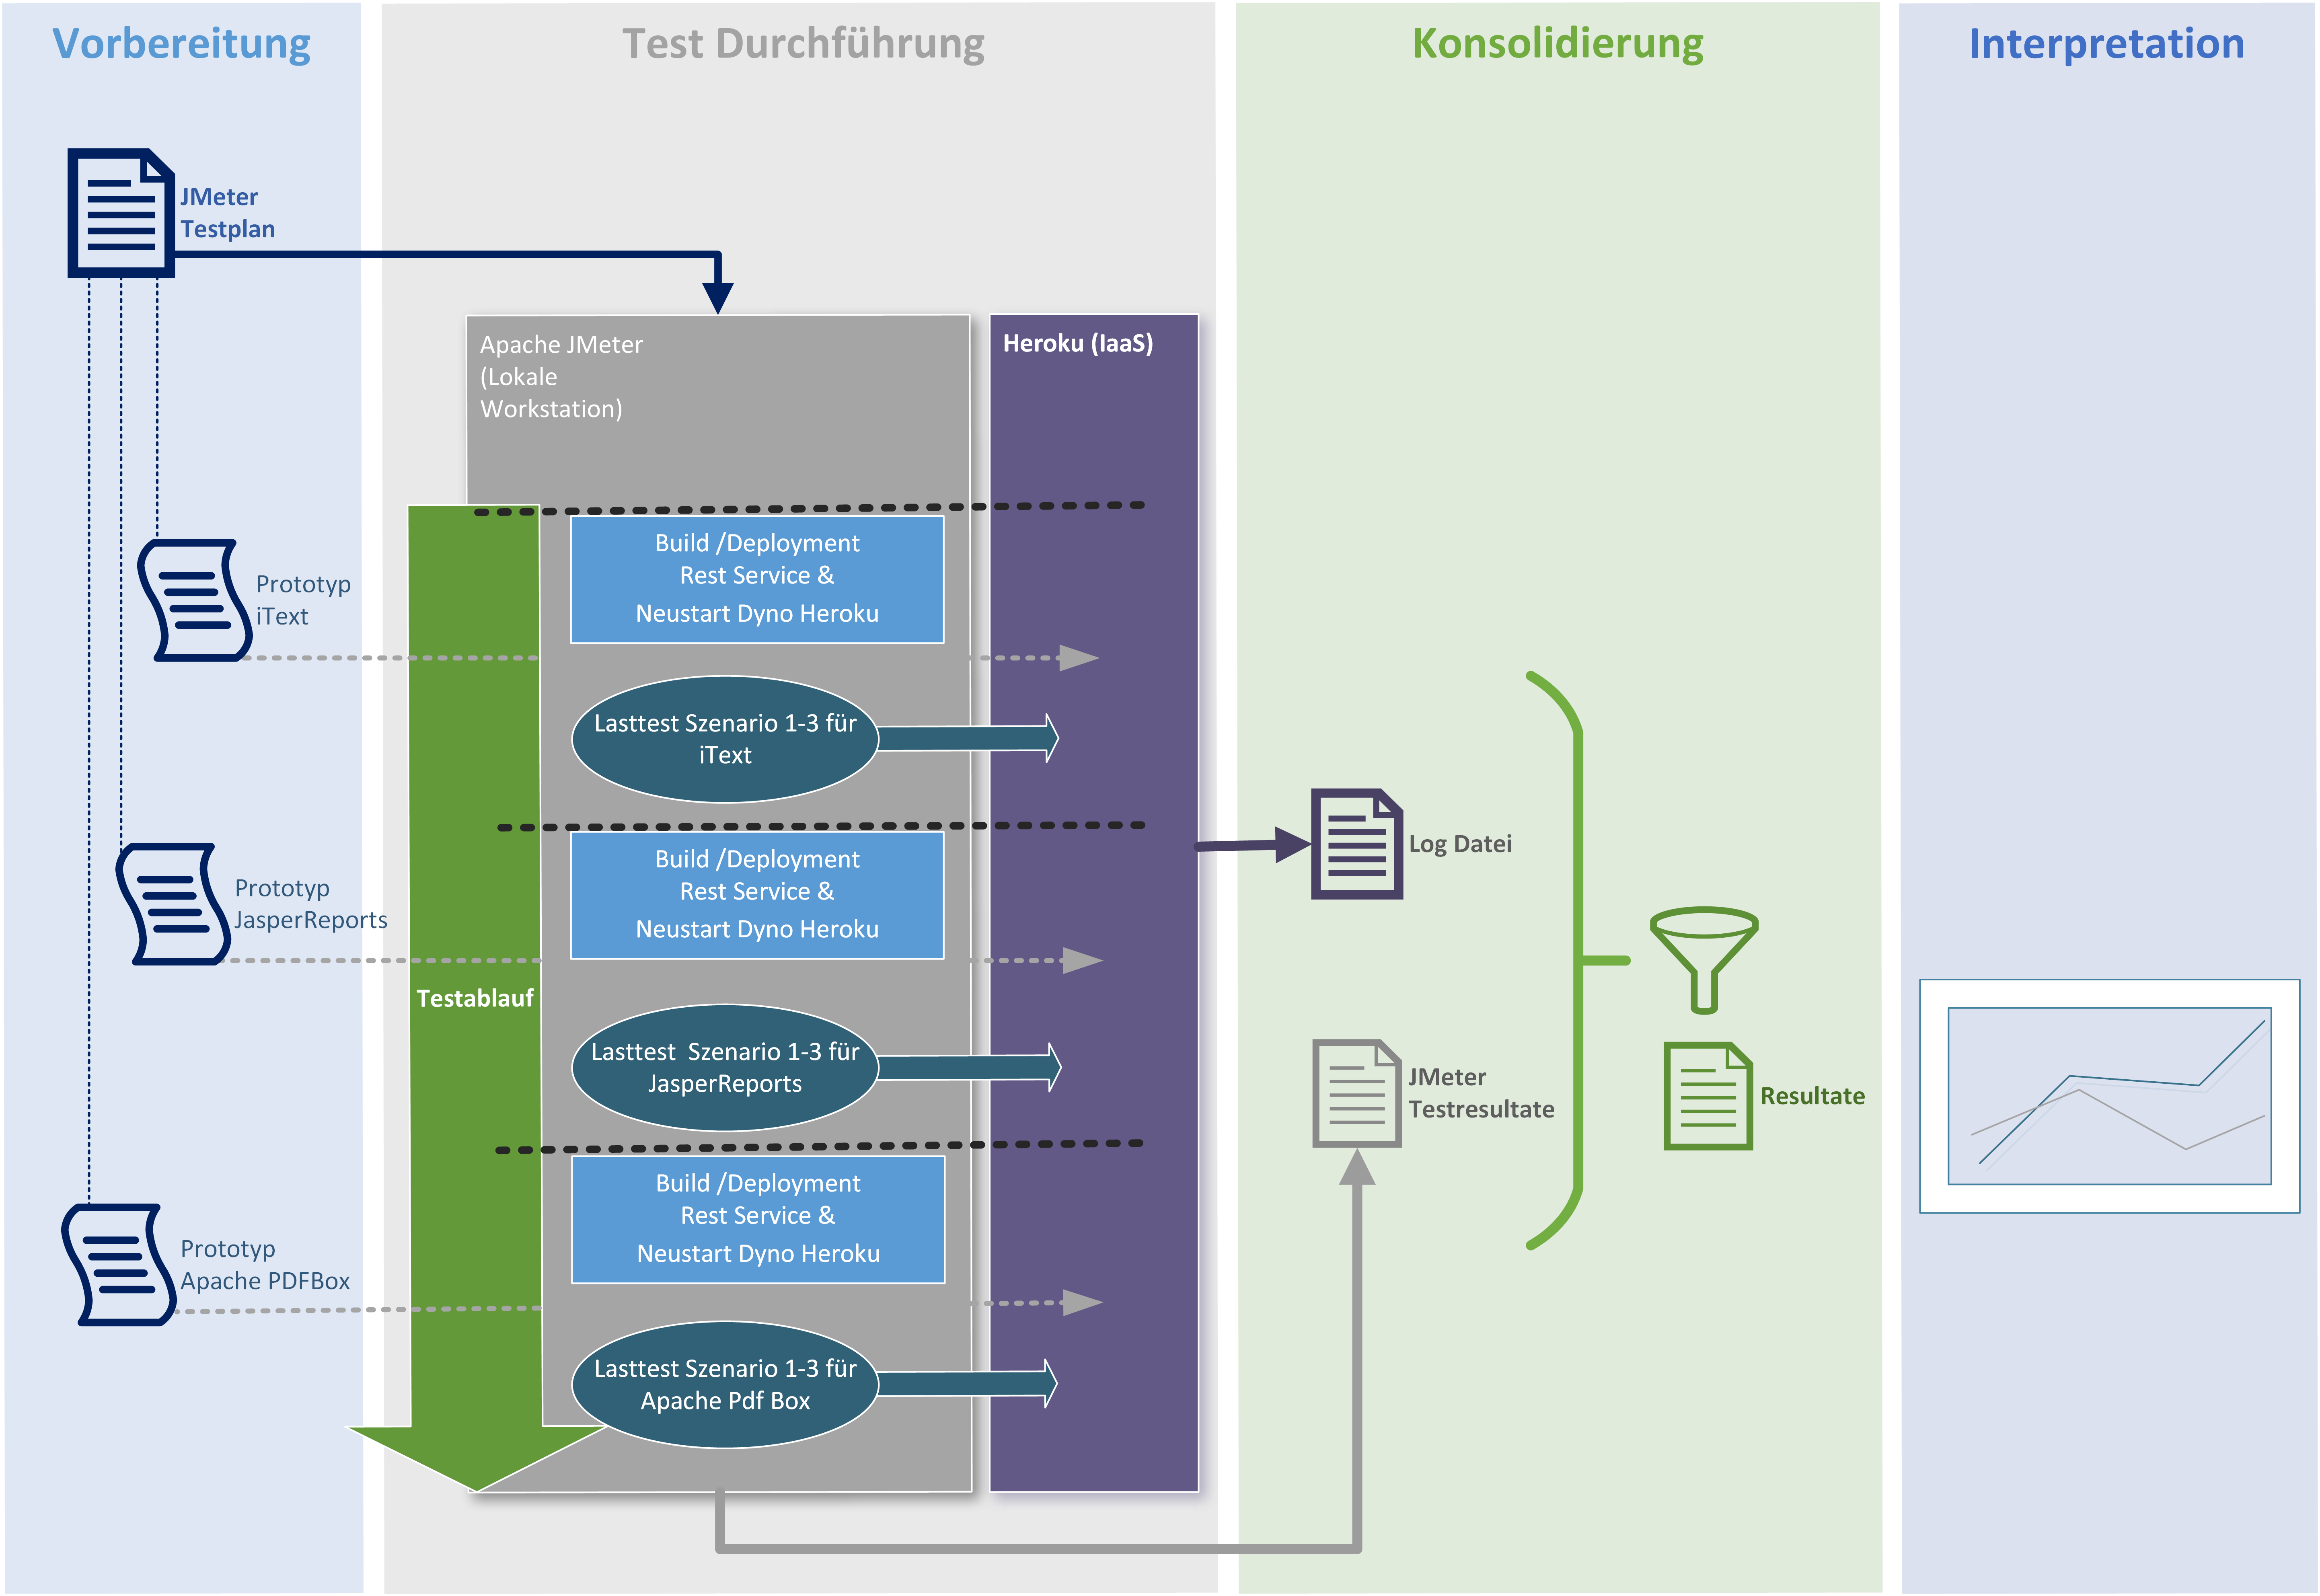
\includegraphics[width=\textwidth]{mainpart/3_methodik_evaluation_img/Testablauf.png}
 \caption{Evaluationsablauf}
 \label{figure:evaluationsAblauf}
\end{figure}


\section{Vorbereitung}
In der Phase Vorbereitung geht es darum, die Prototypen zu erstellen sowie den Testplan zu definieren. 
Im Testplan müssen verschiedene Parameter definiert werden. Wie diese gewählt werden, bestimmt der Anwendungsfall, der hier behandelt wird.

\subsection{Last-Strategie}
Eine Nutzergruppe kann auf ein produktives System verschiedene Last-Muster generieren. Dabei gelingt es den Usern, durch den Ansturm auch grosse Rechenzentren lahmzulegen. Ob alle User gleichzeitig wie z.B. beim Vorverkauf von Konzertkarten beim gebotenen Service anmelden oder gestaffelt, ist für ein System durchaus wichtig, denn je nach Service kann dieser sich mit der Anzahl Anfragen den neuen Umständen anpassen und horizontal skalieren, also die Last auf viele verschiedene Server verteilen.

\subsection{Ramp-Up}
Bei den durchgeführten Lasttest wurde die Infrastruktur nicht skaliert, dennoch wurde eine Ramp-Up von 10 Sekunden definiert, was bedeutet, dass die gesamte Menge der virtuellen User nach 10 Sekunden auf dem System aktiv Last erzeugen. Dieses Szenario wurde gewählt, da in der Praxis fast nie Systeme gleich vollständig ausgelastet werden.

Da es in diesen Experimenten darum geht, verschiedene Anwendungen und deren Frameworks zu evaluieren, wurde eine fixe Anzahl User definiert, die sich über 10 Sekunden hinweg alle zuschalten und 10 Minuten lang auf dem System 'arbeiten'. Somit variieren diese über den Test hinweg nicht mehr. Diese Strategie wurde gewählt, da es einfacher ist, die Messungen zu evaluieren, und die Performance-Messungen zuverlässiger gesammelt werden können. 

\subsection{Last}
Ein Service kann auf verschiedene Arten belastet werden. Einserseits, was öfter vorkommt, ist es das Ansteigen der aktiven User auf dem System. Diese Last wird meist über einen Scale out der Server behoben. Was ebenfalls vorkommt, ist, dass die Last auf dem Service durch grössere Anfragen gefordert wird, d.h. dass Requestgrössen ansteigen. Das kann z.B bei Services, die eine Bestandeslieferung von Einwohnern entgegennehmen, der Fall sein. Diese Anfrage nimmt oft jährlich zu, oder es ist auch möglich, dass grössere Gemeinden als Kunden dazugezählt werden dürfen. 

In dieser Arbeit wurden die beiden Lasten im Testplan miteinbezogen. Bei den Tests wurden einerseits die virtuellen User von 20 auf 50 gesetzt, und andererseits wurden die virtuellen User bei 20 belassen, aber die Requestgrösse verdreifacht. D.h. die zu verarbeitenden Datensätze wurden verdreifacht, nicht die Bytegrösse der Anfragen. Diese Tests sollen Aufschluss darüber geben, wie sich die OSREs bei Lasterhöhung verhalten.

Die definierten Parameter und Testpläne wurden als jmx-Datei festgehalten und für die Testdurchführung aufbereitet.

\begin{reference}{JMeter Testplan}
Der Basisplan kann im Anhang gefunden werden oder unter: 
 \url{https://github.com/denisbittante/dinf/tree/master/loadtest/jmeter/DinfLoadTest.jmx}
 
\end{reference}



\section{Test Durchführung}


Um die Performance einzelner Implementationen testen zu können, wurde eine Serie von Tests erstellt. Die Performancetests spiegeln die Anforderungen an die Services wieder. Dabei wurden verschiedene Parameter verändert, die in der Praxis ebenfalls anzutreffen sind. Im Folgenden werden diese erläutert.

\subsection{JMeter}


Um die definierten Testszenarien durchzuführen, wurde das Open Source Tool Apache JMeter (v.3.3) genutzt. Es gibt eine ganz Reihe von Lasttest- und Performancetest-Software auf dem Markt wie HP LoadRunner, Silk Performer, LoadUI und viele mehr. JMeter wurde ausgewählt, da es ein kostenloses und das am meisten genutzte Last- und Performance-Tool ist. Das Tool unterstützt eine Reihe verschiedener Protokolle, unter anderem REST, was für dieses Experiment genutzt wurde. Die Testszenarien wurden im "Non-GUI oder "headless"-Mode durchgeführt. Dieser dient dazu, intensive Testreihen in einer \acrshort{cli}-Umgebung durchzuführen. Um die Tests durchzuführen, wurde für das Speichern der Ergebnisse folgendes Skript erstellt:

\begin{lstlisting}[language=command.com]

@echo off
for /f "tokens=2 delims==" %%a in ('wmic OS Get localdatetime /value') do set "dt=%%a"
set "YY=%dt:~2,2%" & set "YYYY=%dt:~0,4%" & set "MM=%dt:~4,2%" & set "DD=%dt:~6,2%"
set "HH=%dt:~8,2%" & set "Min=%dt:~10,2%" & set "Sec=%dt:~12,2%"

set "datestamp=%YYYY%%MM%%DD%" & set "timestamp=%HH%%Min%%Sec%"
set "fullstamp=%YYYY%-%MM%-%DD%_%HH%-%Min%-%Sec%"

jmeter -n -t C:/sandbox/dinf/dinf/loadtest/jmeter/LoadTest-TIMED.jmx -l C:/sandbox/dinf/dinf/loadtest/jmeter/testlog-%fullstamp%.jtl

\end{lstlisting}




\begin{reference}{JMeter}
JMeter ist ein Open Source Tool und kann direkt bei Apache heruntergeladen werden. \newline
\url{http://jmeter.apache.org/}
\end{reference}



\subsection{Test Szenarien}
Es wurden verschiedene Szenarien definiert, die einerseits einen möglichen Anwendungsbereich von OSRE abbilden könnten, andererseits sich an den speziellen Implementationen oder Limitierungen der OSRE orientieren. Als Beispiel verfügt Apache PDF Box nicht über eine integrierte Schnittstelle, um Tabellen zu implementieren. Im Folgenden werden diese Szenarien detailliert vorgestellt. 


\begin{reference}{PDF Resultate}
 Die originalen PDFs können auf GitHub oder im Anhang nachgeschlagen werden: \url{https://github.com/denisbittante/dinf/tree/master/doc/results/pdf}
 
\end{reference}

\subsubsection{Szenario 1 - Aktivität}

\begin{figure}[h]
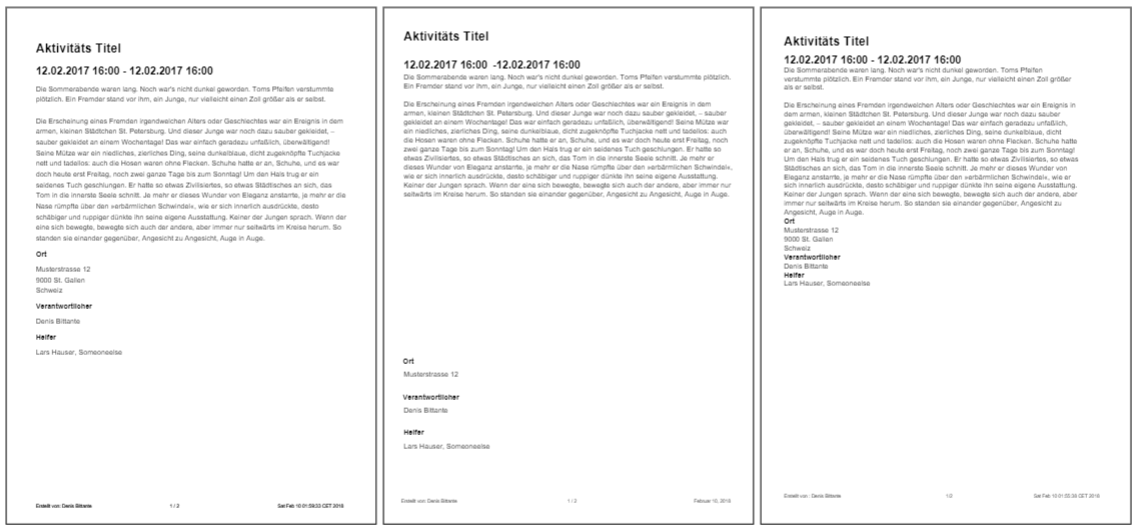
\includegraphics[width=\textwidth]{mainpart/3_methodik_evaluation_img/Szenario1PDF.PNG}
 \caption{PDF-Resultate Szenario 1 (v.l.n.r iText, JasperReports, Apache PDFBox)}
 \label{figure:PDFResultSzen1}
\end{figure}


Im ersten Szenario (siehe Abbildung \ref{figure:PDFResultSzen1}) ging es darum, einen Report wiederzugeben, der in einem Referenzprojekt genutzt wird. Die Anforderung dabei war, einen einfachen Report zu erstellen, der eine Reihe von Aktivitäten oder Terminen abbildet. Dabei wurde darauf geachtet, dass alle s diese Anforderung erfüllen können. Einerseits wurden die Schriftart gewählt und andererseits das Format der Überschriften sowie die Reportgrösse (DIN A4) definiert. Alle Implementationen mussten auch die PDF-Metadaten befüllen, wie die Felder Stichwörter, Autor und Titel. Eine weitere Anforderung für das erste Szenario waren Fussnoten, die es zu implementieren galt.

Die Informationen, die auf den Reports dargestellt werden, spiegeln die Requests wieder. Jeder Eintrag im Request löst dabei eine neue Seite im Report aus, da Apache PDFBox nicht in der Lage war, Floating-Layouts zu erstellen. Somit werden 10 bis 30 Seiten pro Test generiert. Dieser Report soll frei von rechenintensiven Kalkulationen sein, damit gezeigt werden kann, was die s unter optimalen Bedingungen leisten könnten.
 


\subsubsection{Szenario 2- Zeitplan}
\begin{figure}[h]
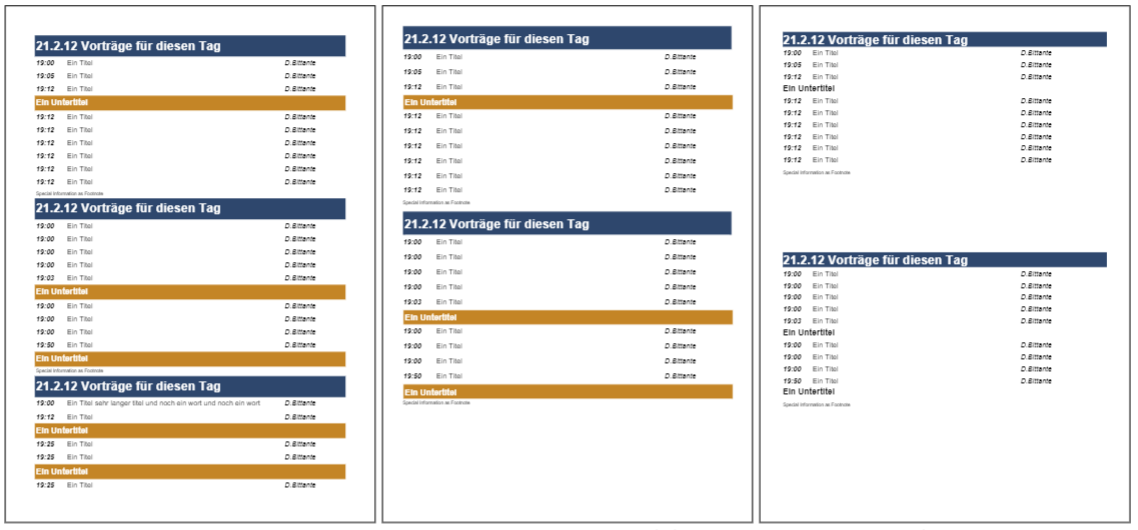
\includegraphics[width=\textwidth]{mainpart/3_methodik_evaluation_img/Szenario2PDF.PNG}
 \caption{PDF-Resultate Szenario 2 (v.l.n.r iText, JasperReports, Apache PDFBox)}
 \label{figure:PDFResultSzen2}
\end{figure}

Im zweiten Szenario wurde ein eher aufwendiges Design erstellt. Der Report bildet einen Zeitplan ab mit verschiedenen Aktivitäten oder Terminen, gruppiert nach Tag. Jeder Tag besitzt dabei ein Datum und einen passenden Titel. Diese Titelzeile galt es farblich hervorzuheben (siehe Abbildung \ref{figure:PDFResultSzen2}). Was das Layout anbelangt, wurden verschiedene Anforderungen definiert, um es etwas anspruchsvoller zu gestalten. Die Tagesabschnitte besitzen je eine Tabelle mit den einzelnen Aktivitäten, auf drei Spalten aufgeteilt. Wird im Request das Flag \texttt{isSubtitle} als \texttt{'true'} gesendet, wird der Untertitel ebenfalls farblich im gelb-orangen Farbton hervorgehoben. Auch Kursiv und Fett im Schriftzug wurde eingesetzt. Das PDF wurde auch hier mit den nötigen Metadaten versehen. An dieser Stelle ist hervorzuheben, dass als Ziel nicht eine perfekte Darstellung der PDF-Reporte im Vordergrund stand, sondern ein möglichst ähnliches und vergleichbares Ergebnis zu erzielen. Auch hier sind Unterschiede festzustellen. Als grober Unterschied ist ApachePDFBox aufzuführen, bei der die Hervorhebung des Untertitels in Farbe zu aufwendig wurde. Da der Hintergrund der Titelzeile als Box gezeichnet wird, mussten die entsprechenden Koordinaten angegeben werden. Um den Hintergrund eines Untertitels anzugegeben, hätte man die Berechnung der Koordinaten in Bezug auf die Font-Grösse durchführen müssen, was nicht mehr zielführend war.

In diesem Anwendungsfall gilt es zu prüfen, wie eine OSRE mit komplexem Seitenaufbau zurechtkommt und wie sich das auf die Performance auswirkt und vor allem, wie die Ressourcen dabei genutzt werden. Dabei soll der Seitenaufbau komplizierter sein. Die Datenmengen werden im Test zwischen 10 und 30 Datensätzen sein, was zu einer PDF-Länge von vier (iText) bis maximal 15 Seiten führt.

\subsubsection{Szenario 3 - Kontaktliste}

\begin{figure}[h]
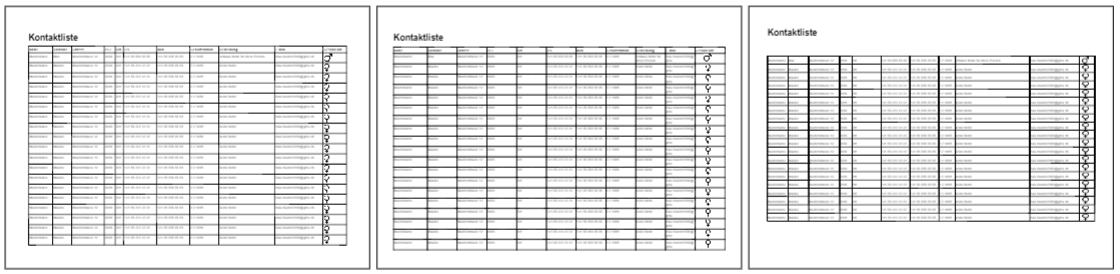
\includegraphics[width=\textwidth]{mainpart/3_methodik_evaluation_img/Szenario3PDF.PNG}
 \caption{PDF-Resultate Szenario 3 (v.l.n.r iText, JasperReports, Apache PDFBox)}
 \label{figure:PDFResultSzen3}
\end{figure}

In diesem Anwendungsfall soll gezeigt werden, welche OSRE am besten geeignet wäre, Bilder in einem Report zu verarbeiten. Dieser Anwendungsfall generiert zwar nur Reports, die ein bis zwei Seiten lang sind, diese müssen aber dennoch möglichst schnell generiert werden. Der definierte Anwendungsfall kann in der Abbildung \ref{figure:PDFResultSzen3} gesehen werden. Das definierte Ziel war eine Übersicht der Kontakte, die z.B. im Zusammenhang mit den Aktivitäten eingeladen hat. Es wurde definiert, dass diese Übersicht erneut die nötigen Metadaten befüllt, auch Fusszeilen auf den PDFs dürfen nicht fehlen. Das interessante in diesem Anwendungsfall war die Verarbeitung der Bilder. Die Bilder waren in einer hohen Auflösung abgelegt und mussten skaliert und gegebenenfalls komprimiert werden. Des Weiteren wurde definiert, dass sich die Seite im Querformat zu orientieren hat und der Titel nur auf der ersten Seite anzuzeigen ist.

Die zu erzeugenden Tabellen wurden von den s verschieden implementiert, wie in der Einführung bereits angesprochen wurde. In iText lässt die Tabellenfunktion einzelne Zellen erstellen und mit JasperReports konnte die Tabelle als Subreport oder sogar als Datensatz formatiert werden. Apache PDFBox war in dieser Hinsicht etwas primitiv. Die Tabelle wurde in der Grösse berechnet und jedes Feld wurde einzeln auf der Arbeitsfläche hinzugefügt. Anschliessend wurden die Felder mit gezeichneten Strichen umrandet.




\section{Konsolidierung}
In diesem Schritt der Evaluation geht es darum, die Daten zu vereinheitlichen und zu konsolidieren.

\subsection{Log Datei}

Die Daten, die Heroku niederschreibt, sind unter anderem die eingehenden Requests, der Dyno Load und der Memoryverbrauch. Diese Daten werden als Zeichenketten in die Loggs geschrieben. Nicht gesteuert von den Aktivitäten auf dem Dyno, sondern aufgrund eines Timers werden diese Daten aus einer Probe des Dynos gelesen und in die Logs persistiert. Um diese Daten auswerten zu können, wurde ein eigener Log Parser geschrieben, mit welchem es möglich ist, diese Logs zu finden und in einer eigenen kommaseparierten Datei zu speichern.

\begin{reference}{Log Extractor Source Code}
Der Log Extractor kann hier gefunden werden:  \url{https://github.com/denisbittante/dinf/tree/master/loadtest/utils/src/ch/ffhs/dinf/utils/log}
 
\end{reference}



\subsection{JMeter Testresultate}


Die Ergebnisse von JMeter können wiederum im selben Tool im Gui-Modus gelesen und ausgewertet werden. Dazu bietet JMeter verschiedene Auswertungmethoden an. Einerseits können Plug-In’s weitere Aufbereitungsmethoden zur Verfügung stellen, oder sonst sind mit JMeter bereits ein Dutzend Aggregatoren und grafische Tools mit dabei. Des Weiteren wurde Microsoft Excel genutzt, um die Daten in grafischer Form aufzubereiten.

\begin{reference}{Konsolidierte Daten}
Die Konsolidierten Daten können hier heruntergeladen werden:  \url{https://github.com/denisbittante/dinf/tree/master/loadtest/results}
 
\end{reference}









\end{document}